\documentclass{sig-alternate-05-2015}
\usepackage{graphicx}
\graphicspath{ {images/} }

\begin{document}


\title{Citi Bike share analysis}  
\subtitle{[Project Report - 061]}
\subtitle{\url{https://gitlab.com/cloudmesh_fall2016/project-061.git}}

\numberofauthors{1} 

\author{
\alignauthor
Aruna Kumaraswamy\\
F16-DG-4034\\
       \affaddr{Indiana University}\\
       \email{akumaras@iu.edu}
}
\date{09 December 2016}

\maketitle

\begin{abstract}
    Purpose of this project is to analyze the NYC Citi Bike share system data in batch and streaming mode. Following report summarizes the finding based on the September 2016 bike share data. Report will also provide instructions on installing the necessary software, build and deploy the software created for this project.    
\end{abstract}


\section{Introduction}
Apache Flink is used in this project to process the data in batch and streaming mode. 

\subsection{Proposed Design}
\begin{figure}[!ht]
\includegraphics[width=8cm, height=5cm]{pipeline}
 \caption{CitiBike project - Data pipeline}\label{F:small}
\end{figure}

There are 4 stream components.
\begin{itemize}
    \item CitiBikeStreamToKafka
    \item AllRidesFromKafka
    \item PopularBikeStationFromKafka
    \item LiveStationStatusStream
\end{itemize}
\break
There are 2 main batch components in this project
\begin{itemize}
    \item BikeRentTrendByAge
    \item BikeRentTrendByGender
\end{itemize}
Components are built in Java. Maven is used for building the components.
\subsection{Citi Bike Stream To Kafka}
Citi Bike publishes trip history per month in S3 as zip files. This component will use the zip source and stream the data via Kafka for archiving to a sink and also analysing in real time via slicing window the popular stations. So the data has to be published to 2 topics. 

\subsection{All rides from Kafka}
This streaming flink job is a consumer of kafka topic ridesToTableSink. Proposed solution was to use data sink such as HBase. Due to time constraints, I have used CSV sink for analysis.

\subsection{Popular BikeStations From Kafka}
This streaming flink job is a consumer of kafka topic ridesToWindow. It counts the rides within a 15 minute data chunk and slices to 5 minute window for streaming analysis. If the ride count is more than 50 for a start station, then it is considered a popular station.

\subsection {Bike Rent Trend - By Age}
Objective of this analysis is to find in which age group bike share is popular. This component takes csv file as input. For age group analysis, we are interested only in the age, so we skip all the other columns in the spreadsheet. Based on the age group, we decide if the bike rider is Boomer I, Boomer II, Gen X, Gen Y or Gen Z. Invalid age in the data is filtered. Final result is the count of the age groups for September 2016. Figure 2 depicts the visualization for this batch program. Visualization is created using a python program.

\begin{figure}[!ht]
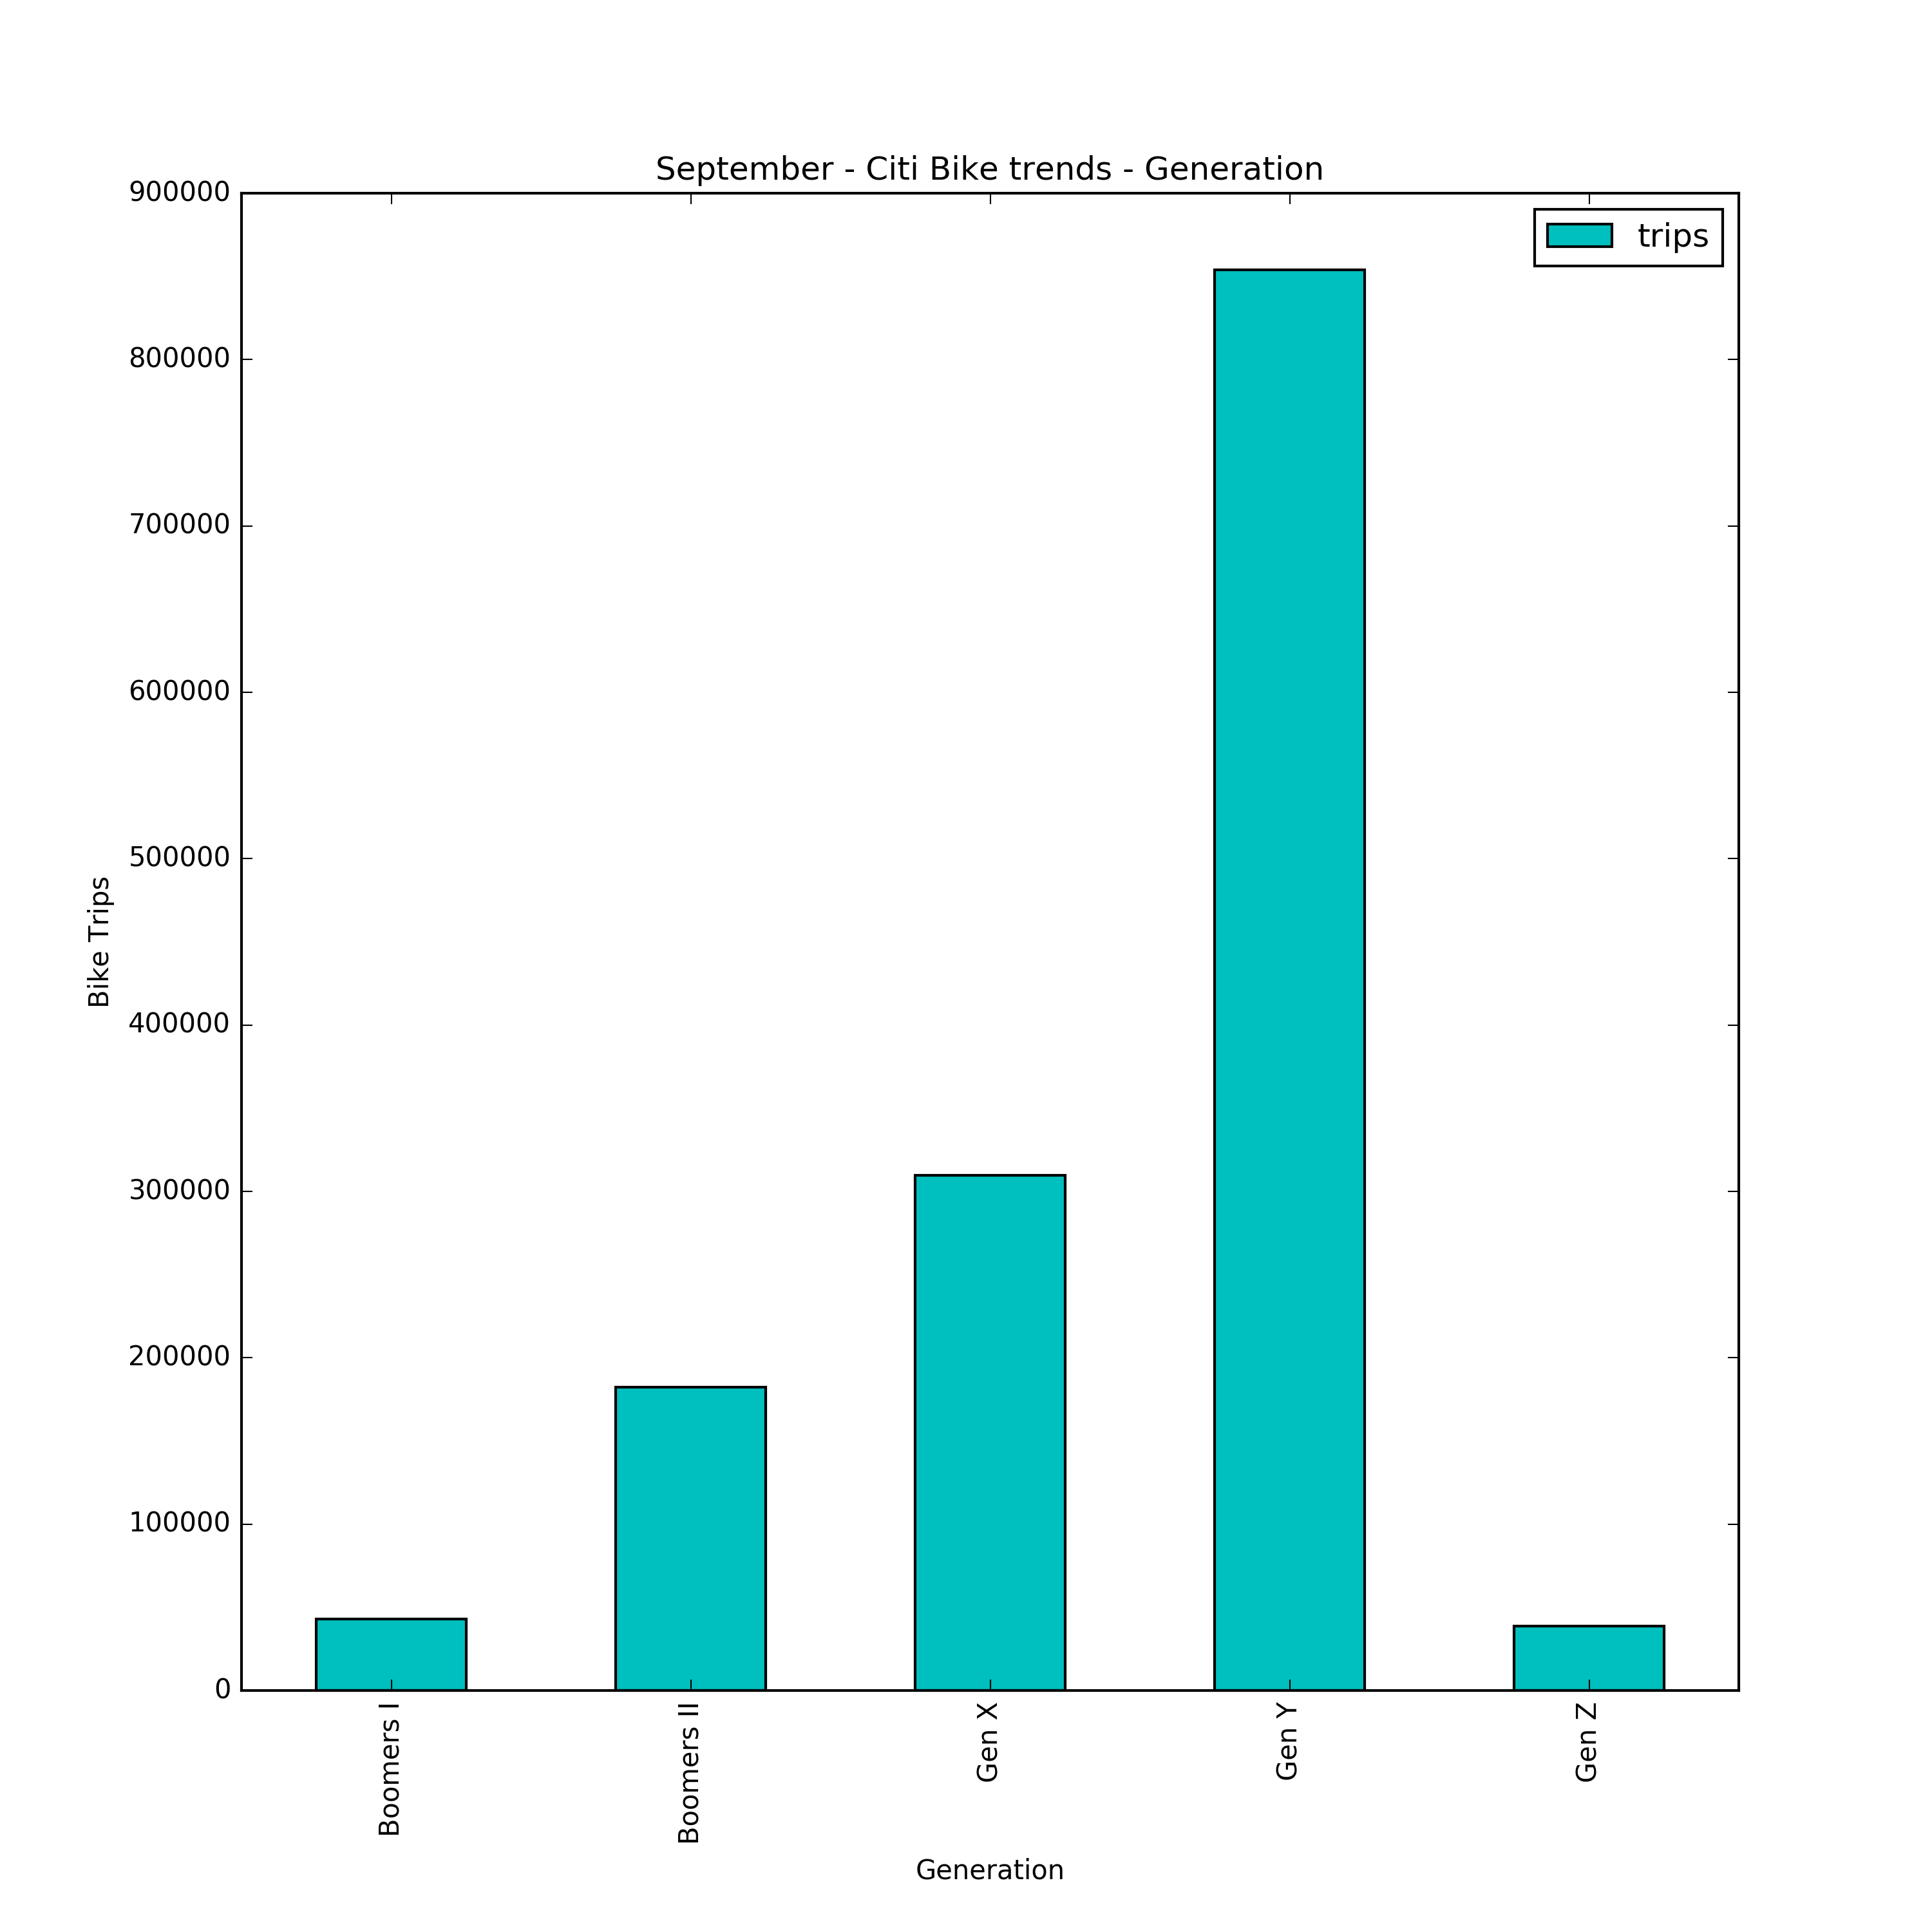
\includegraphics[width=8cm, height=5cm]{tripsbygeneration}
 \caption{Trend By age}\label{F:small}
\end{figure}

\break
\subsection {Bike Rent Trend - By Gender}
Objective of this analysis is to find whether bike ride is popular among men or women. This component takes CSV file as input and creates a CSV output. We are interested in trip date, gender column of the spreadsheet, so we skip other columns. We also filter unknown gender. We transform the input data using tables
and join them to produce the desired CSV output. Figure 3 is the visualization for this batch program. Visualization is created using python program.

\begin{figure}[!ht]
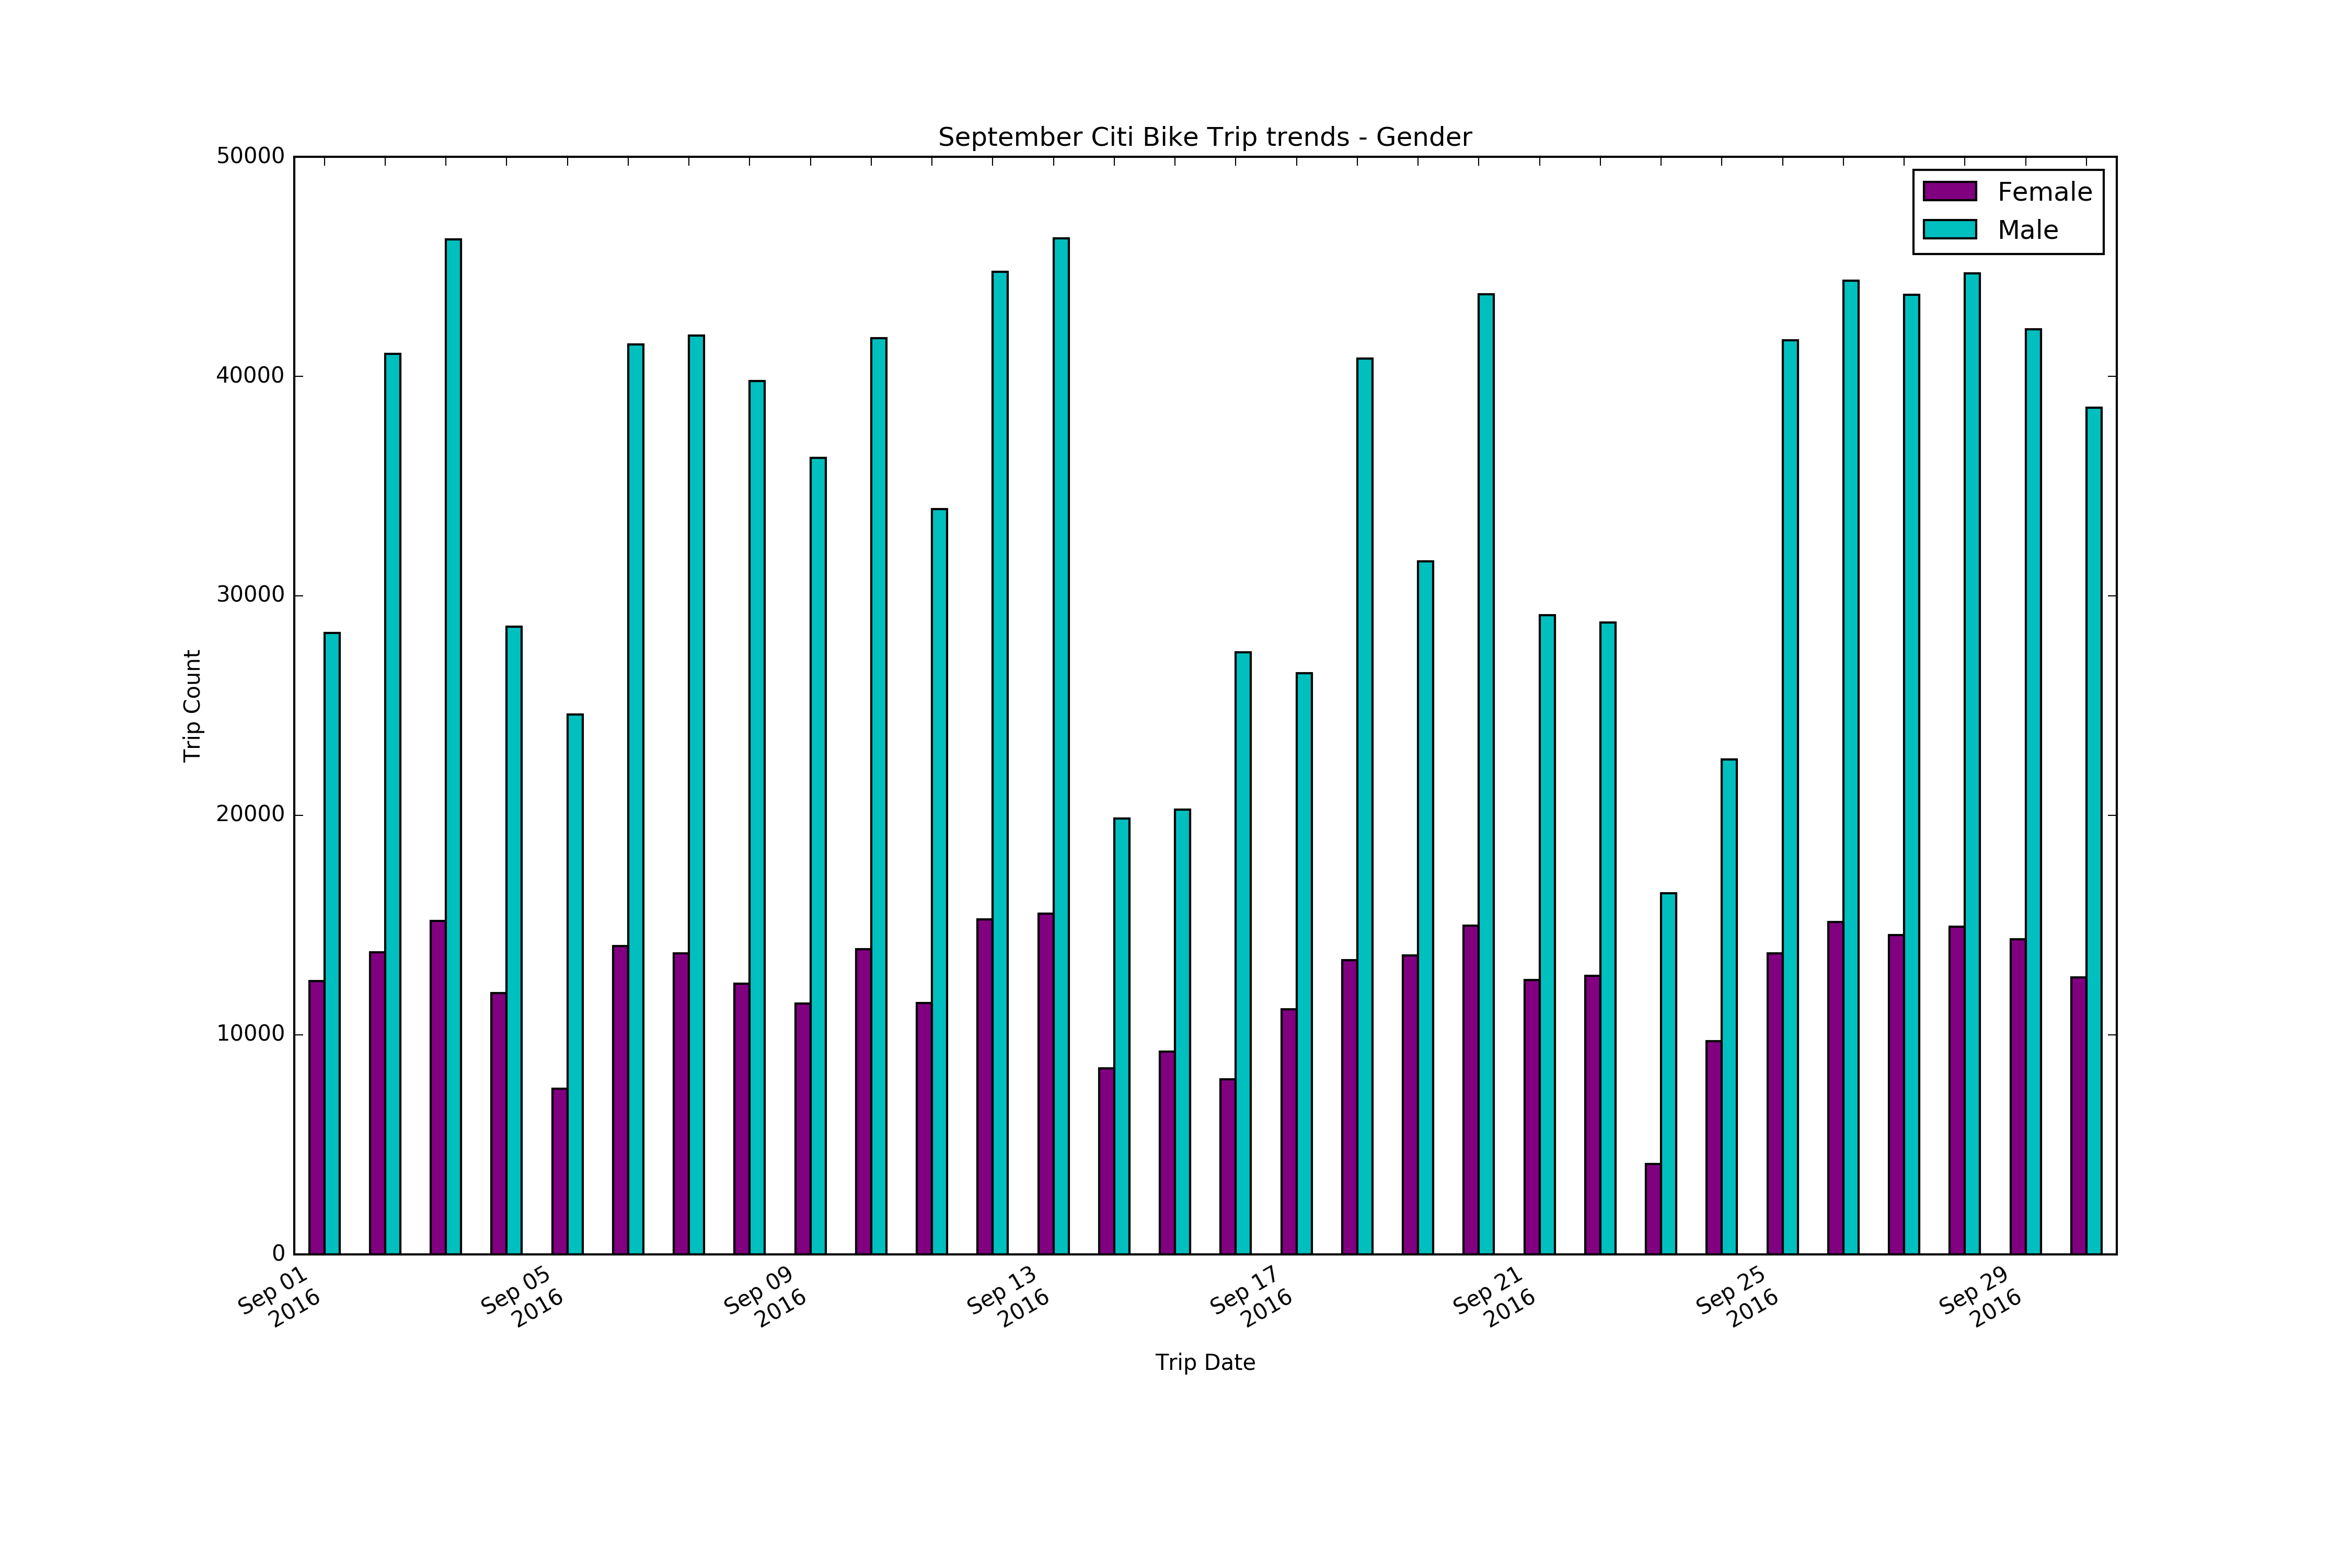
\includegraphics[width=8cm, height=5cm]{tripsbygender}
 \caption{Trend By gender}\label{F:small}
\end{figure}
\subsection {Live Station Status Stream}
Live station status feed is used to check the availability of bikes across all stations. If the bike availability of a station is less than 2 then those stations are filtered. Result is pushed to elastic search. Kibana is used for visualization of real-time alerts across geographic map. Figure 4 is a representation on Geo map done via Kibana.

\begin{figure}[!ht]
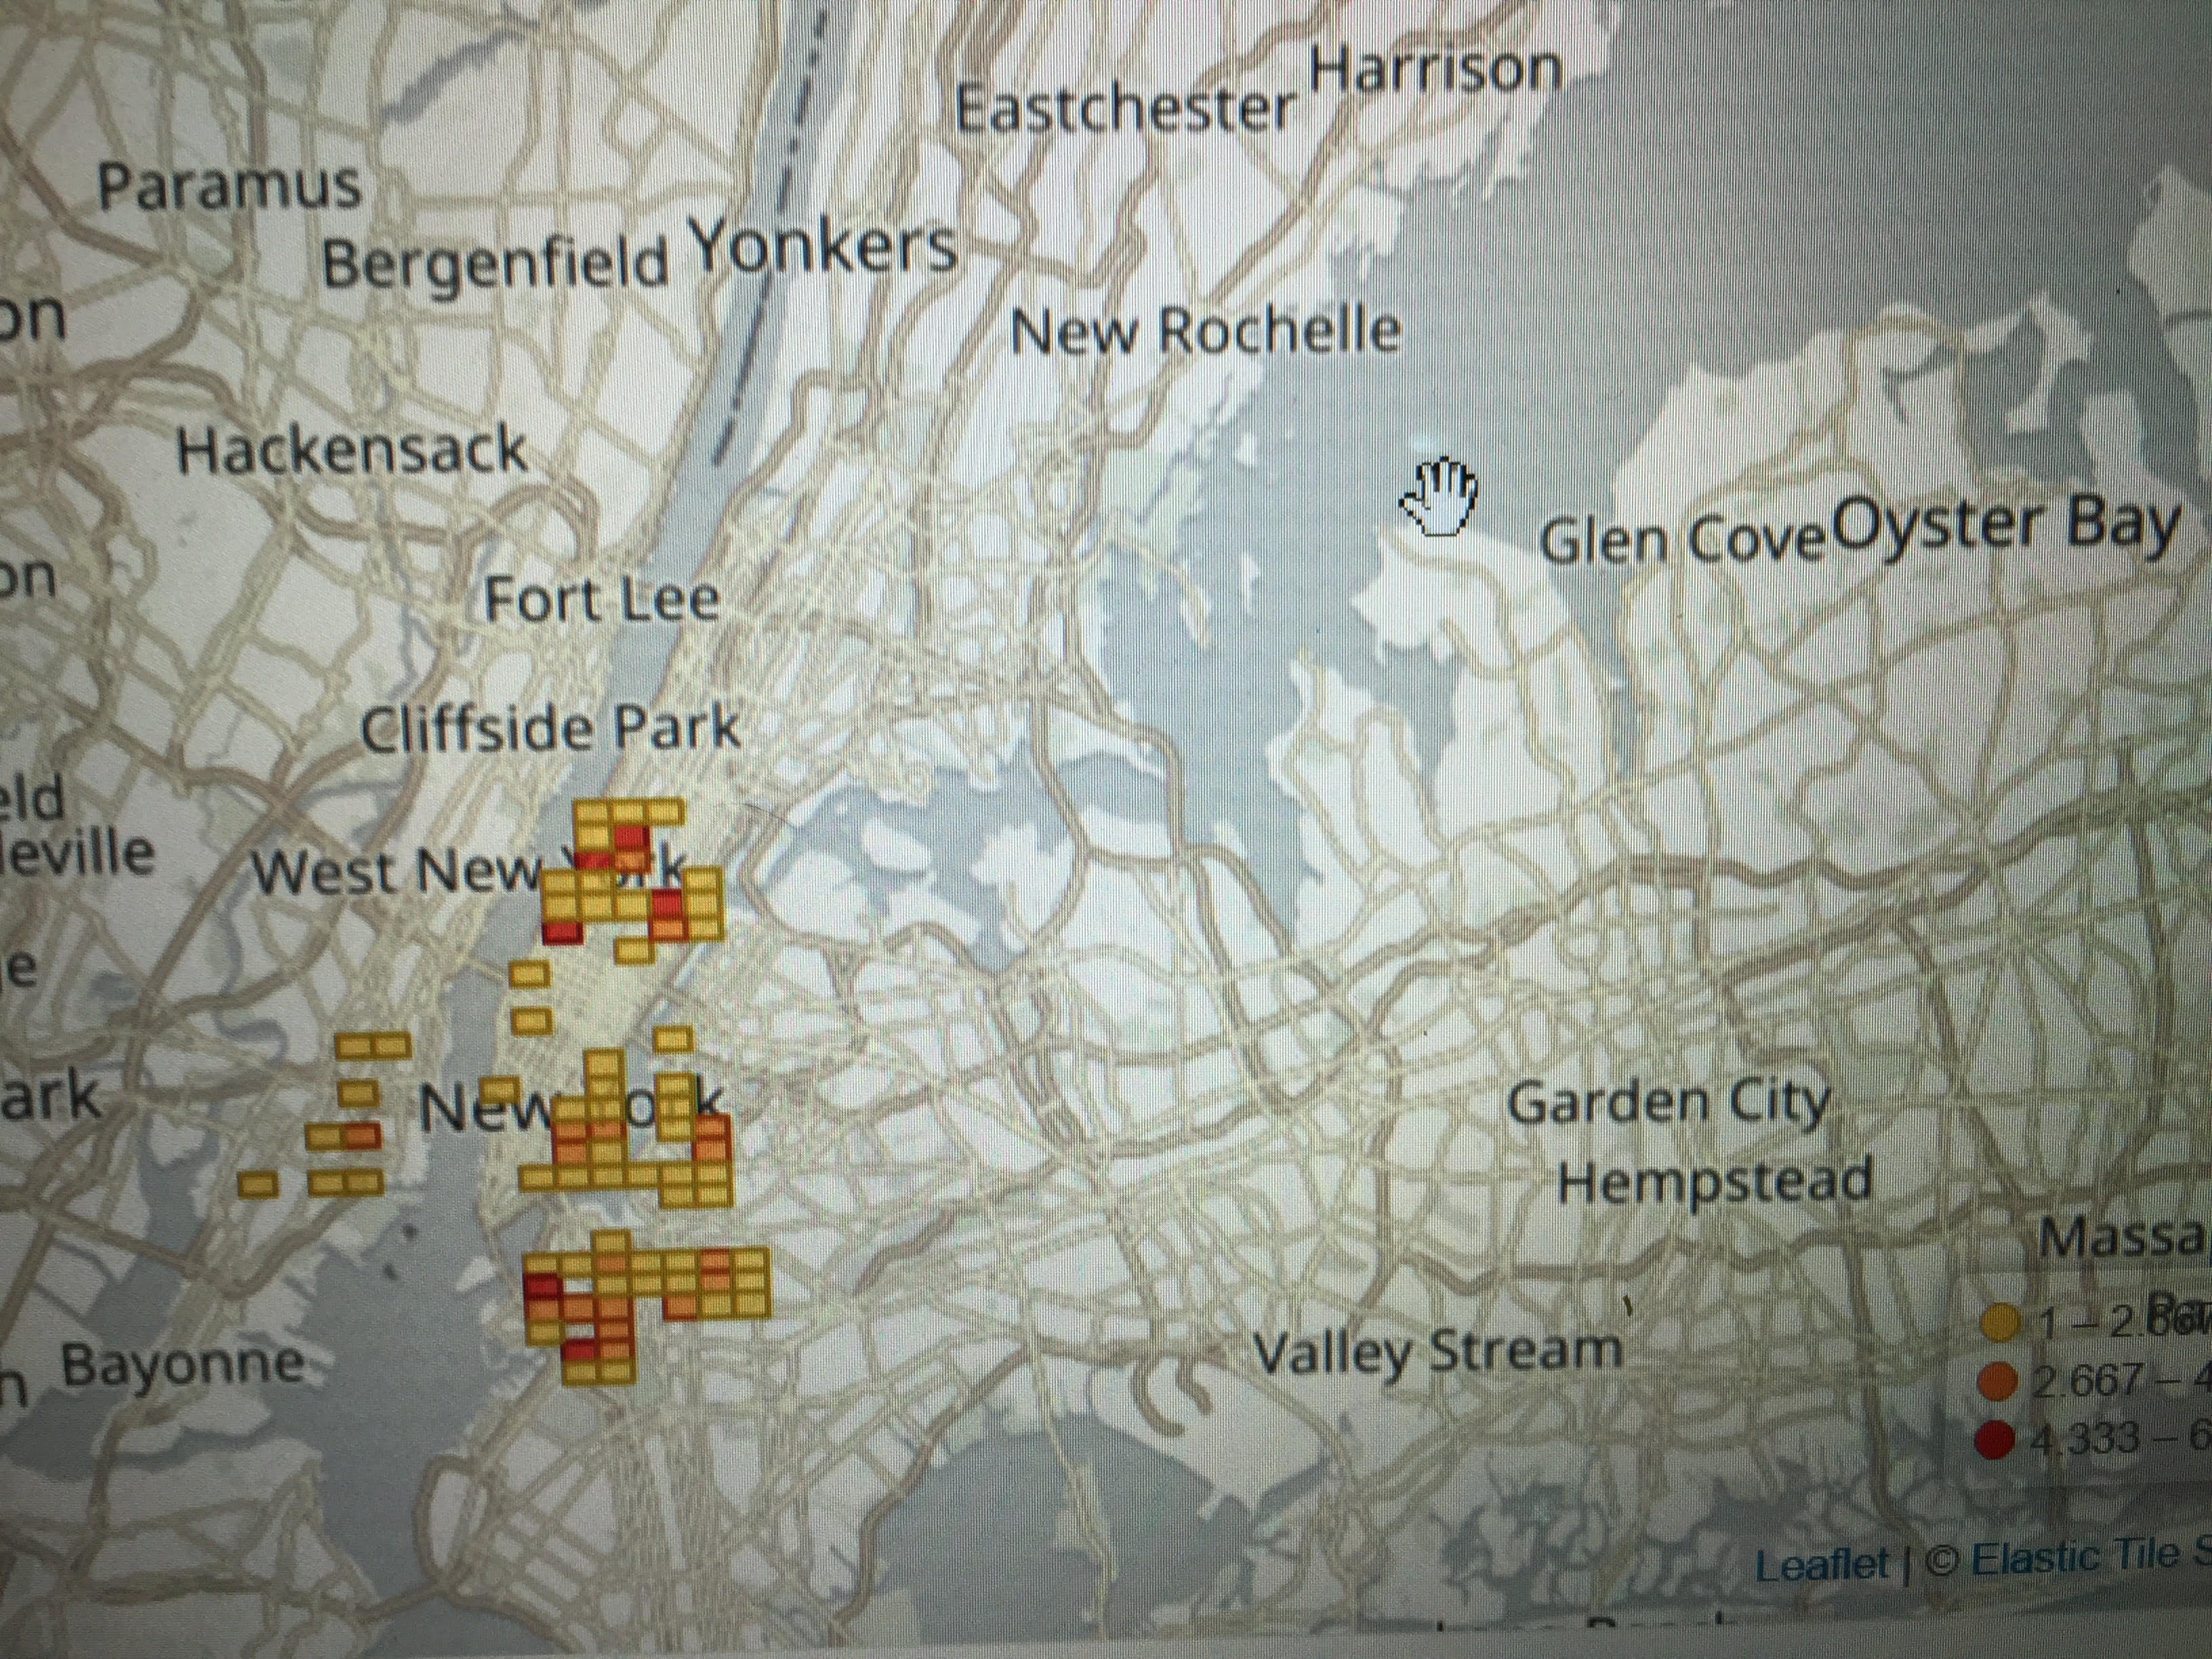
\includegraphics[width=8cm, height=5cm]{bikealerts}
 \caption{Bike alerts}\label{F:small}
\end{figure}


\section{Technology}


\subsection{Apache Flink}
When I wrote the initial proposal for this project, I was planning to use Spark. I was interested in deploying a lambda architecture using spark and kafka. More I read about flink, it became obvious that flink is ideal for both batch and streaming data. Even though sparks supports streaming, it is usually a micro batch.

\cite{kjacobs} Figure 5 and Figure 6 shows the comparison between spark and flink.

\begin{figure}[!ht]
\includegraphics[width=8cm, height=5cm]{disk-spark_flink}
 \caption{Spark Vs Flink Disk I/O}\label{F:small}
\end{figure}

\begin{figure}[!ht]
\includegraphics[width=8cm, height=5cm]{spark_flink_latency}
 \caption{Latency comparison spark vs flink}\label{F:small}
\end{figure}
\break
\break

\subsection{Kafka}
Kafka is used to establish the data pipeline between Flink jobs.


\subsection{Elastic search and Kibana}
In this project I am using elastic search and Kibana for streaming visualization. It is based on the training on flink by data artisan \cite{artisan}. Elastic search indexes are created via curl or Kibana appsense. LiveStationStatusStream component fetches data from bike share realtime feed. It can be modified to continuously fetch real time data. Current implementation is to show the behaviour of data streaming via real time feed. This data is cleansed, filtered and sent to Elastic search sink specifying the index we created via curl. Kibana can now be used to setup indexes, time characteric and search to display the bike alert data in geo map. Kibana does not allow download of the visualization, hence the   of kibana is submitted in this report.


\section {Installation}
Flink - Install flink version 1.1.3 \break
Kafka - Install kafka_2.10-0.9.0.1\break
Elastic search - Install version 2.3.5\break
Kibana - 4.5.4 (with appsense plugin)\break
Python 2.7\break

\section {Build and Deploy}

Clone GIT repository

\subsection {Step1 Build Java code}
Build java code using \break
mvn clean package

\subsection {Step2 Prepare data}
Use wget or bitsadmin to get trips data from \break
https://s3.amazonaws.com/tripdata/201609-citibike-tripdata.zip
\break
Flink is unable to process ZIP directly. So unzip the data file.

\subsection{Step 5 Kafka}
Start Zookeeper
Start Kafka

\subsection {Step 4 Elastic Search Index}
Start Kibana
Go to http://localhost:5601/appsense
Create the citi-bikes index (Refer data instruction in GIT)
Start Elastic Search


\subsection {Step 5 Run Flink}
Refer to README.rst in GIT for detailed instructions on how 
to run batch and stream processing components in Flink.
\break
\break

\section {Conclusion}
Apache Flink offered ease of use and better performance to perform analysis in batch environment. SQL processing in batch mode simplifies data preparation and storage.
\break
Stream Execution environment has rich set of features and connector. Even though Table API is same for batch and stream, I had difficulty getting Kafka stream to dump to a table sink.   
\break
Flink does not have a REST API similar to Spark to submit jobs, hence creating a web dashboard would take more effort.
\break
Parallelism and Task slot configuration has to be adjusted in flink to run jobs concurrently.
\break
AllRidesFromKafka writes the BikeRide attributes to csv sink in a different order. Hence I am unable to use that sink as input for the batch jobs.


\bibliographystyle{abbrv}
\bibliography{report} 
\end{document}
